\chapter{The \fshark{} Wrapper}
In this chapter we will first demonstrate how to compile and use an \fshark{}
module within an \fsharp{} project.
Then, we will explain the \fshark{} Compiler and it's pipeline.

mere here

Although \fshark{} code can be executed directly in \fsharp{} as normal
\fsharp{} code, our benchmarks in chapter \ref{chap:evaluation} shows
that compiling our \fshark{} code to Futhark OpenCL modules gives us performance
increases by several orders of magnitudes (from $\times 100~\text{to}~\times 1000$).

\section{Using the \fshark{} Wrapper}
\label{sec:fsharkcompiler}

\subsection{Another short \fshark{} module}
\begin{figure}[H]
  \centering
\begin{minted}[linenos]{fsharp}
module ExampleModule
open FSharkPrelude

let saxpy (a : int) (x : int) (y : int) : int =
  a*x+y

let getArrayPair (a : int) : (int array * int array) =
  let xs = Iota a
  let n = Length xs
  let ys = Rotate (n / 2) xs
  in (xs, ys)

[<FSharkEntry>]
let entry (a : int) : int array =
  let (xs, ys) = getArrayPair a
  let res = Map2 (saxpy a) xs ys
  in res
\end{minted}
  \caption{A short \fshark{} module in a file named ExampleModule.fs}
  \label{fig:fsharkusageexample0}
\end{figure}

In figure \ref{fig:fsharkusageexample0} we see a simple \fshark{} module that we
want to compile into a GPU kernel and use in our \fsharp{} program.
\\
Line by line, this module does the following:\\
\textbf{L1:} We define the name of this module as \texttt{ExampleModule}. If we
want to use this module in an \fsharp{} program without compiling it as
\fshark{} first, we can refer to this module by this name.
\\
\textbf{L2:} We open \fshark{}s standard library \texttt{FSharkPrelude} in this
module, so we can access the standard functions in the \fshark{} module.
In this module, we are using the standard functions \texttt{Iota}, \texttt{Length}, \texttt{Rotate} and \texttt{Map2}.
\\
\textbf{L4-5:} We define the function \texttt{saxpy}.
\\
\textbf{L7-11:} We define the function \texttt{getArrayPair}.
\\
\textbf{L8:} \texttt{Iota a} returns the integer array of the numbers from $0$
up to, but not including, $a$.
\\
\textbf{L9:} \texttt{Length xs} returns the length of the array \texttt{xs}.
\\
\textbf{L10:} \texttt{Rotate n} rotates the contents of an array n places in
either the right or left direction.\\
In example, \texttt{Rotate 2 [1;2;3;4;5;6] = [5;6;1;2;3;4]},\\
and \texttt{Rotate (-2) [1;2;3;4;5;6] = [3;4;5;6;1;2]}
\\
\textbf{L11:} Here we return the pair of arrays \texttt{(xs, ys)}.

\textbf{L13-17:} We define the entry function \texttt{entry}.\\
\textbf{L15:} We call \texttt{getArrayPair} to get two arrays.\\
\textbf{L16:} We use \texttt{Map2} to map the curried function \texttt{(saxpy
  a)}
over the arrays \texttt{xs} and \texttt{ys}.

For two arrays $\mathtt{xs} =
[\mathtt{x}_1,~\mathtt{x}_2,~\ldots,~\mathtt{x}_n]$ and $\mathtt{ys} =
[\mathtt{y}_1,~\mathtt{y}_2,~\ldots,~\mathtt{y}_n]$,\\
$\mathtt{Map2}~\mathtt{(saxpy~a)}~\mathtt{xs}~\mathtt{ys} = [\mathtt{saxpy~a}~\mathtt{x}_1~\mathtt{y}_1, \mathtt{saxpy~a}~\mathtt{x}_2~\mathtt{y}_2,\ldots,~\mathtt{saxpy~a}~\mathtt{x}_n~\mathtt{y}_n]$.
\textbf{L17:} The entry function returns the result of the call to \texttt{Map2}.

This concludes the short \fshark{} module.
\clearpage

\subsection{Compiling and using the short \fshark{} module}
\label{compilingandusingfsharkmodule}
With our \fshark{} module ready, we now proceed to compile, load and use it.
\begin{figure}[h]
  \centering
    \begin{minted}[linenos,breaklines]{fsharp}
module FSharkExample
open FShark.Main

[<EntryPoint>]
let main argv =
  let wrapper = 
    new FSharkWrapper(
      libName="ExampleModule",
      tmpRoot="/home/mikkel/FShark",
      preludePath= "/home/mikkel/Documents/fshark/FSharkPrelude/bin/Debug/FSharkPrelude.dll",
      openCL=true,
      unsafe=true,
      debug=false
      )
  wrapper.AddSourceFile "ExampleModule.fs"
  wrapper.CompileAndLoad
  let a = 1000000
  let result = wrapper.InvokeFunction("entry", a) :?> int array
  printfn "Mapping (+2) over %A gives us %A" xs xs'
  0
    \end{minted}
  \caption{An F\# program using \fshark{}}
  \label{fig:fsharkusageexample}
\end{figure}

\textbf{L6:} We begin by constructing an instance of the \fshark{}Wrapper. It has the following
mandatory arguments:

\begin{description}
\item[\texttt{libName}]\hfill\\
  This is the library name for the \fshark{} program. In the final Futhark
  \texttt{.cs} and \texttt{.dll} files, the main class will have the same name
  as the \texttt{libName}. This doesn't really matter if \fshark{} is just used
  as a JIT compiler, but it's good to have a proper name if the user only wants
  to use the compiler parts of \fshark{}.

\item[\texttt{tmpRoot}]\hfill\\
  The \fshark{} compiler works in its own temporary directory. This argument must
  point to a directory where F\# can write files and execute subprocesses
  (Futhark- and C\# compilers) which also has to write files.
  
\item[\texttt{preludePath}]\hfill\\
  The \fshark{} compiler needs the FShark prelude available to compile FShark
  programs. 

\item[\texttt{openCL}]\hfill\\
  Although Futhark (and therefore \fshark{}) is most effective on OpenCL-enabled
  computers, the benchmarks in \ref{sec:benchmarks} still show a significant
  speed increase for non-OpenCL Futhark over native F\# code.
  Therefore, \fshark{} is also available for non-OpenCL users. Use this flag to
  tell \fshark{} whether Futhark should compile C\# with or without OpenCL.
  
\item[\texttt{unsafe}]\hfill\\
  For some Futhark programs, the Futhark compiler itself is unable to tell
  whether certain array operations or SOAC usages are safe, and will stop the
  compilation, even though the code should (and does) indeed work.
  To enable these unsafe operations, pass a \texttt{true} flag to the compiler.

\item[\texttt{debug}]\hfill\\
  Passing the debug flag to the \fshark{} compiler enables various runtime
  debugging features, for instance benchmarking the time it takes to run various
  parts of the compiler.
\end{description}

\textbf{L15:} Now we can pass a source file to the \fshark{} wrapper. \\
\textbf{L16:} We tell the wrapper to compile the source file that we have added
to the wrapper object, and load the compiled library into the wrapper
afterwards.
\textbf{L17:} As our entry function defined in the module in figure
\ref{fig:fsharkusageexample0} takes an integer as argument, we define an integer
variable we can pass to it.
\textbf{L18:} We use the wrapper to invoke the entry function from the compiled
and loaded library, using our previously declared \texttt{a} as the only
argument. As the \fshark{} wrapper uses reflection to dynamically load compiled
libraries at runtime, we are not able to statically determine what type of
result we will get from the \texttt{InvokeFunction} call. Therefore, we use F\#s
downcast operator \texttt{(:?>)} to declare the return value as an \texttt{int
  array}.

If we are in doubt of which type to downcast to, we can always lookup the return
type by reviewing the \fshark{} module's source code. We can downcast to any of
the types usable in \fsharp{}, including tuples and arrays.

\section{On the design decisions of the \fshark{} wrapper}
To summarize, the current design of \fshark{} usage is dependent on a
wrapper object, which for all \fshark{} projects must compile and load 
the input \fshark{} modules once, and, afterwards, it must pass arguments 
from \fsharp{} to the resulting GPU kernels by using .NET reflection.
This design has several costs for both usability and performance, and we will
here discuss some of these costs, and what we could do to alleviate them in the
future.

\subsection{Compiling and loading \fshark{} modules at every startup}
At this time, \fshark{} works by compiling and loading \fshark{} modules just in
time before they are needed in the containing \fsharp{} project. However, this
is more often than not redundant work. For the developer who is using \fshark{} to develop
prototypes of \fshark{} GPU kernels, it is of course beneficial to continuously
recompile the \fshark{} program under development to verify that changes are being
made.

However, when the \fshark{} program is finished and ready to be used in
projects, it isn't necessary to compile it again.

\subsubsection{How much time do we spend on compiling and loading the \fshark{} modules?}
If we, instead of loading the compiled \fshark{} GPU kernels through the
\fshark{} wrapper, just open the compiled kernel libraries as any other
\csharp{} \texttt{.dll} file, we can circumvent the \fshark{} compiler
completely, and use the compiled kernel directly.

For the two benchmarks \texttt{LocVolCalib} and \texttt{nbody}(see sec
\ref{benchmarks}), we have compared the time cost of the two different
approaches. In figure \ref{benchmarkcalculations} we see how the time is spent
in the two different methods.
\begin{figure}[H]
  \centering
  \begin{tabular}{@{}l c r c l c r}
 Parsing \fshark{} code using \fsharp{} parser          & &   217984 ms & $\vrule$ & & & \\
    Converting \fsharp{} declarations to FSharkIL       & &+   19129 ms & $\vrule$ & & & \\
 Converting FSharkIL to Futhark source code             & &+   98949 ms & $\vrule$ & & & \\
 Compiling Futhark to \csharp{} with \texttt{futhark-cs}& &+ 8037165 ms & $\vrule$ & & & \\
 Compiling \csharp{} code using \csharp{} compiler      & &+  999251 ms & $\vrule$ & & & \\
 Loading compiled \csharp{} class using reflection      & &+  101601 ms & $\vrule$ & & & \\
 Loading and constructing class from library & & & $\vrule$ & & &
  \end{tabular}
  \caption{Time spent on making LocVolCalib available in \fshark{}-using
    program}
  \label{benchmarkcalculations}
\end{figure}

So the dynamic compilation process takes about $10$ seconds, while running the
accelerated program on the largest dataset takes only a couple of seconds.

MORE BENCHMARKS

WE ARE OBVIOUSLY WASTING TIME

\subsubsection{Suggestions for changes}
We have two main suggestions for change.\\
1) The easiest way would be to add a \texttt{AddModulePath} function to the
\fshark{} wrapper. The benchmarks show that we aren't spending that much more
time when loading compiled assemblies into \fsharp{} using reflection, than if
we opened the assembly as a library in the project.

Therefore, we could add a function that takes a path to a compiled \fshark{}
module, and loaded the path's target into the wrapper.

2) We could also go for a second, more permanent solution. Instead of relying on
\fsharp{}s reflection functionality to load our compiled assemblies into scope
dynamically, we could redesign the \fshark{} use case itself, so that it uses
just the compiler, and not the wrapper.

In this case, the new use case would be to compile the \fshark{} modules using
the \fshark{} compiler, and then manually reference- and open them in \fsharp{} projects.
This would not only remove the repeated module compilation, but also let us use
static typing with the compiled \fshark{} modules, enabling autocompletion and
type checking for function arguments, and also removing the need to manually
downcast the \fshark{} invokation results.

\subsection{The overhead of invoking GPU kernels}
The second issue with the current approach is, that every single call to a
\fshark{} function carries significant overhead for copying data back and forth
between CPU and GPU buffers.
This is a problem when we are chaining together GPU function calls: that is when
we take the array output of function $f$ and use it as an argument for function
$g$ without any changes to it.

In figure \ref{fig:witharraycopying} we see a chain of three calls to a compiled \fshark{} module. 
Although we are calling the second function with the result from the first
function together with another array, and calling the third function with result
from the second function, we are still moving the results from the GPU buffers to our system RAM between each call, and deallocating
the buffers on the GPU, even though we are going to reallocate them soon
thereafter.

\begin{figure}[H]
  \centering
  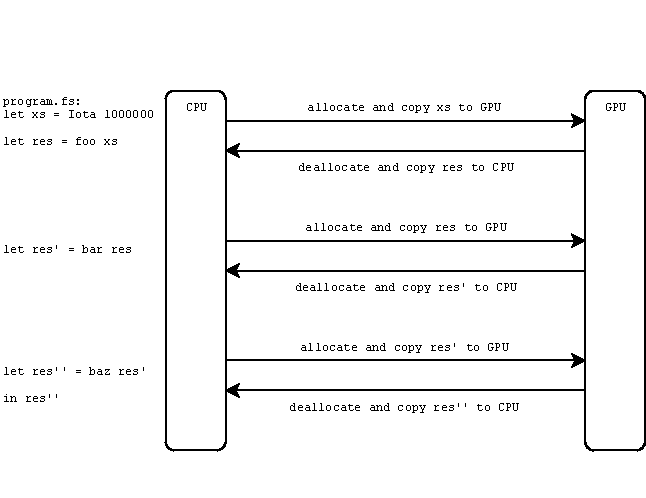
\includegraphics[scale=1.15]{chapters/figs/witharraycopying.pdf}
  \caption{Buffers are copied back and forth between CPU and GPU between calls}
  \label{fig:witharraycopying}
\end{figure}


In the future, we could eliminate this overhead by allowing the compiled Futhark functions
to return references to GPU buffers instead of indiscriminately returning
actual data arrays.
We could then also have multiple versions of the compiled Futhark functions; one
version that takes an actual data array as input, and one that can use a
reference to a GPU buffer instead.

In this case, we could wait until after the three function calls to actually
copy the referenced GPU buffer back to the system RAM. This would strongly reduce the
number of copies back and forth between the GPU and the system RAM:
Instead of the allocations/deallocations increasing linearly with the number of
chained GPU kernel calls, we can make do with one allocation and one
deallocation between system RAM and GPU, pr. chain, as in figure \ref{fig:withoutarraycopying}
\begin{figure}[H]
  \centering
  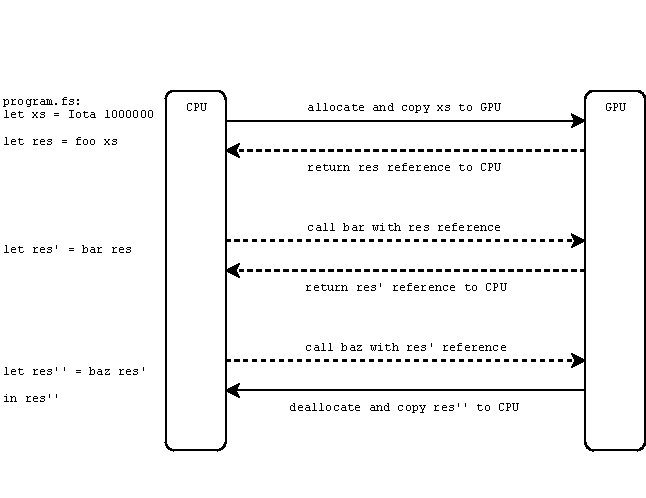
\includegraphics[scale=1.15]{chapters/figs/withoutarraycopying.pdf}
  \caption{Buffers aren't copied between CPU and GPU unless necessary}
  \label{fig:withoutarraycopying}
\end{figure}

This functionality is already implemented in Python's \texttt{PyOpenCL} library,
and is used in Futhark programs that are compiled as Python libraries.
\clearpage

\chapter{The \fshark{} Compiler}
At this point in the report, we are able to generate GPU-accelerated
computational kernels for \csharp{}. We
have also defined a language for writing GPU kernels using \fsharp{}, and we have
offered several methods of integrating these compiled \csharp{} kernels in
\fsharp{} projects. What remains is to build a compiler, that takes \fshark{}
code as input, and returns a compiled \csharp{} library that runs GPU
computational kernels.

In practice, we need to build an architecture that supports the functionality
defined in figure \ref{fig:fsharkcompilerarchitecture}.

\begin{figure}[H]
  \centering
  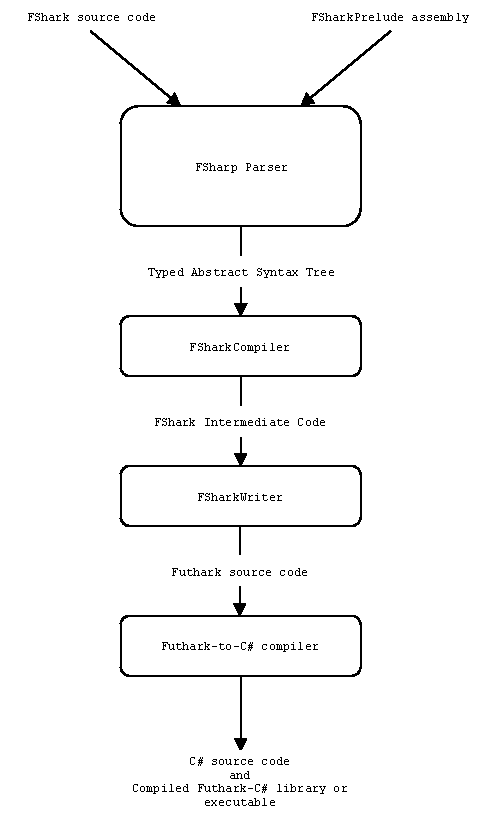
\includegraphics[scale=1.15]{chapters/figs/compilerarchitecture.pdf}
  \caption{The complete architecture from \fshark{} source code to compiled
    \csharp{} program.}
  \label{fig:fsharkcompilerarchitecture}
\end{figure}


\section{The FSharp parser}
Parsing and building a regular \fsharp{} program is trivial when using official build tools like
\texttt{msbuild} or \texttt{fsharpc}.
But in the case of \fshark{}, we are not interested in the final output of the
\fsharp{} compiler. Instead, we use only part of the \fsharp{} compiler's
pipeline: By passing our \fshark{} source code through the \fsharp{} compiler's
parser features, we retrieve its corresponding Typed Abstract Syntax Tree.

The Typed Abstract Syntax Tree (TAST) contains the function and value declarations that makes up 
our \fshark{} program.
The Typed Abstract Syntax Tree is merely an AST that already has tagged all the
contained expressions with their respective types.\\
We take this TAST and pass it on into the \texttt{FSharkCompiler}.

As the F\# Software Foundation offers the official F\# Compiler as a freely
available NuGet package for F\# projects, we can use this package
\texttt{FSharp.Compiler.Services} to parse the entire input \fshark{} program and
give us a Typed Abstract Syntax Tree of the FSharp expressions therein, instead
of writing our own parser. So as the \fsharp{} parser part of the pipeline amounts to calling some library
functions from an imported library, we will not use more time on this part.

\section{The \fshark{}Compiler}
For the \fshark{}Compiler, we need to build a module that takes an \fsharp{}
TAST as input, and returns the corresponding program as written in an
intermediate language defined for \fshark{}, called \fshark{}IL.\\
The declarations in the TAST are called \texttt{FSharpDecl}s, and in \fshark{}
we work with two kinds of \texttt{FSharpDecl}s.

The first kind is the \texttt{FSharpDecl.Entity}. Entities are \fsharp{}
declarations that are neither functions or values
themselves, but instead alterations to the present \fsharp{} program. 
The \fshark{}Compiler supports three different entities.

The other kind of FSharpDecl that \fshark{} supports is the \texttt{FSharpDecl.MemberOrFunctionOrValue}, which are
declarations of members, functions and values. We don't use members in
\fshark{}, as they are for object oriented \fsharp{} programming, but we do use
functions and values. For all intents and purposes, \fsharp{} values are just
functions without arguments.

\subsection{FSharpDecl.Entity}
The \fshark{}Compiler supports three different entities.
\begin{description}
\item[FSharpRecords] are standard record types, and can be translated to
  Futhark records with ease.
  This entity has an empty \texttt{FSharpImplementationFileDeclaration list}.
\item[FSharpAbbreviations] are type abbreviations, and are easily translated
  into Futhark type aliases.
  This entity has an empty \texttt{FSharpImplementationFileDeclaration list}.
\item[FSharpModules] are named modules which contains subdeclarations. In
  \fshark{} we don't support parameterized modules, so in reality the just work
  as namespaces for functions and values.
  The \fshark{} compiler supports building FShark modules, but current
  limitations demands that modules are flattened when compiled to Futhark.
  This also means that function name prefixes in function calls are stripped
  when compiled to Futhark.

  An example of this module flattening is shown in
  figure \ref{fig:moduleflattening}. Here, the \texttt{Vec3} module is flattened
  and made part of the outer scope of the file. 
  Due to time constraints, this current solution was chosen.
  The solution does introduce the danger of namespace collisions. I.e.,
  we could get in trouble by having a function further down in figure
  \ref{fig:moduleflattening} which was also called \texttt{plus}.

  A later version of the \fshark{}Compiler could very well contain a better
  solution to the module problem, either by translating \fshark{} modules to
  Futhark modules, or at least by naming the flattened module declarations in a
  special way; i.e. by keeping the containing module's name in the flattened
  declarations' name, like in figure \ref{fig:moduleflattening'}.
\end{description}

\begin{figure}[H]
  \centering
\begin{minted}{fsharp}
module Vec3 =
    type Vec3single = {x:single ; y:single ; z:single}
    let plus (a : Vec3single) (b : Vec3single) : Vec3single =
        {x=a.x+b.x; y=a.y+b.y; z=a.z+b.z}
            
type vec3 = Vec3.Vec3single
type mass = single
type position = vec3
type acceleration = vec3
type velocity = vec3
\end{minted}

\begin{lstlisting}[language=Futhark]
type Vec3single = {x : f32, y : f32, z : f32}
let plus (a : Vec3single) (b : Vec3single) : Vec3single =
  {x=((a.x + b.x)), y=((a.y + b.y)), z=((a.z + b.z))}

type vec3 = Vec3single
type mass = f32
type position = Vec3single
type acceleration = Vec3single
type velocity = Vec3single
\end{lstlisting}
  \caption{An \fshark{} module is flattened when compiled to Futhark}
  \label{fig:moduleflattening}
\end{figure}

  
\begin{figure}[H]
  \centering
\begin{minted}{fsharp}
module Vec3 =
    type Vec3single = {x:single ; y:single ; z:single}
    let plus (a : Vec3single) (b : Vec3single) : Vec3single =
        {x=a.x+b.x; y=a.y+b.y; z=a.z+b.z}
            
type vec3 = Vec3.Vec3single
\end{minted}

\begin{lstlisting}[language=Futhark]
type Vec3_Vec3single = {x : f32, y : f32, z : f32}
let Vec3_plus (a : Vec3_Vec3single) (b : Vec3_Vec3single) : Vec3_Vec3single =
  {x=((a.x + b.x)), y=((a.y + b.y)), z=((a.z + b.z))}

type vec3 = Vec3_Vec3single
\end{lstlisting}
  \caption{A better way of flattening modules, so that the risk of name
    less An \fshark{} module is flattened when compiled to Futhark}
  \label{fig:moduleflattening'}
\end{figure}

\subsection{FSharpDecl.MemberOrFunctionOrValue}
HMMMM MERE HER.

In total, this means that our intermediate language must also support four
different declarations, which are the \texttt{FSharkDecl}s. These are shown in
figure \ref{fig:fsharkdecls}.

\begin{figure}
  \centering
\begin{tabular}{@{}l c l}% to \linewidth {l c X}
  $Decl$ & $:=$    & $\lit{FSharkRecord}([(field_1, decl_1),\ldots,(field_n, decl_n)])$ \\
         & $\vert$ & $\lit{FSharkTypeAlias}(name, \tau)$ \\
         & $\vert$ & $\lit{FSharkModule}(name, [decl_1,\ldots, decl_n])$\\
         & $\vert$ & $\lit{FSharkVal}(name, [\tau_1, \ldots, \tau_n], [arg_1, \ldots, arg_n], \tau_{return}, e)$\\
  ~ \\
\end{tabular}
\caption{The four possible \texttt{FSharkDecl}s.}
\label{fig:fsharkdecls}
\end{figure}

\subsection{\fsharp{} expressions}
\label{sec:fsharpexprs}
An \fsharp{} function or value is not without its accompanying \fsharp{}
expression. The \fsharp{} compiler compiles these \fsharp{} expressions into
\texttt{FSharpExpr}s, which we can parse ourselves, and rewrite as \fshark{}IL expressions.
In figure \ref{fig:fsharpexprs0} we see three different \fsharp{} expressions,
and their representations as \texttt{FSharpExpr}'s.

For the first example, we just create a tuple literal. In the
\texttt{FSharpExpr} version, we see how the literal is created using
\texttt{NewTuple}. \texttt{NewTuple} takes a list of \texttt{FSharpExpr}s as
arguments. In this case, we are using two constants, each of which takes some
primitive object, and the .NET type of that object.

In the second example, we use the \texttt{Let} expression. Semantically, \texttt{Let} takes a
name $n$ and two expressions $e_1$ and $e_2$, and exchanges every instance of
$n$ in $e_2$ with $e_1$.
Then we encounter two \texttt{Let}-expressions that we didn't write ourselves.
That is because the \fsharp{} compiler turns tuple assignments into chains of
\texttt{Let} expressions instead. Here, we use \texttt{TupleGet} to get each
field of the tuple.

Finally, we use a typed instance of the \texttt{Call} expression to call the
overloaded function \texttt{Plus} as the integer version of the plus function,
giving it the two variables \texttt{Value a} and \texttt{Value b} as arguments.

In the third example, we see the \texttt{Lambda} expression in use. \texttt{Lambda} takes
a list of variables (in the form of name/type pairs), and an \texttt{FSharpExpr}. In this case,
\texttt{Lambda} only has one variable.\\
The innermost expression here is the \texttt{Application} expression.
\texttt{Application} takes a function or a lambda, and a list of arguments, and
applies the list of arguments one by one to the function or lambda.

\begin{figure}[H]
  \centering
\begin{minted}{fsharp}
  // example 1
  (79, 42.0f)

  // example 2
  let tuple = (79, 42.0f)
  let (a,b) = tuple
  in a + a

  // example 3
  let a = 2.0f
  let foo = fun x -> x + 3.0f
  in foo a
\end{minted}

\begin{minted}{lisp}
  ; example 1
  NewTuple ([Const(79, System.Int32), Const(42.0f, System.Single)])

  ; example 2
  Let tuple (NewTuple ([Const(79, System.Int32), Const(42.0f, System.Single)]))
  ( 
    Let a (TupleGet 1 tuple) 
    (
      Let b (TupleGet 2 tuple) 
      (
        Call Plus System.Int32 
          ([Value a, Value b])
      )       
    )
  )

  ; example 3
  Let a Const(2.0f, System.Single)
  (
    Let foo (Lambda ([(x, System.Single)]) 
                   (Call Plus System.Single 
                     ([Value x, Const(3.0f, System.Single)])
                   ))
    (
      Application foo ([Value a])
    )

  )
\end{minted}
  \caption{Three \fsharp{} expressions, and their representation as
    \texttt{FSharpExpr}s}
  \label{fig:fsharpexprs0}
\end{figure}

The entire set of \texttt{FSharpExpr}s used in the \fshark{}Compiler is
available in figure \ref{fig:fsharpexprs1}.

The entire set of .NET types used in the \fshark{}Compiler is
available in figure \ref{fig:fsharptypes0}.

\begin{figure}[H]
  \centering
\begin{tabular}{l c l}% to \linewidth {l c X}
   $\tau$& $=$     &  \texttt{System.Int8} \\
         & $\vert$ &  \texttt{System.Int16} \\
         & $\vert$ &  \texttt{System.Int32} \\
         & $\vert$ &  \texttt{System.Int64} \\
         & $\vert$ &  \texttt{System.UInt8} \\
         & $\vert$ &  \texttt{System.UInt16} \\
         & $\vert$ &  \texttt{System.UInt32} \\
         & $\vert$ &  \texttt{System.UInt64} \\
         & $\vert$ &  \texttt{System.Single} \\
         & $\vert$ &  \texttt{System.Double} \\
         & $\vert$ &  \texttt{System.Boolean} \\
         & $\vert$ &  \texttt{System.Array} $\tau$ \\
         & $\vert$ &  \texttt{System.Tuple} $(\tau_1 \times \ldots \times \tau_n)$ \\
\end{tabular}
\caption{The .NET types used in the \fshark{}Compiler}
\label{fig:fsharptypes0}
\end{figure}


\begin{figure}[H]
  \centering
  \begin{tabular}{@{}l c l}% to \linewidth {l c X}
e & $=$ &   Const(obj, $\tau$) \\
 & $\vert$ &   Value(v) \\
 & $\vert$ &   AddressOf(v) \\
 & $\vert$ &   NewTuple($\_, [e_0,...,e_n]$) \\
 & $\vert$ &   NewRecord(($v_0 : \tau_0 * \ldots * v_n : \tau_n), [e_0,...,e_n]$) \\
 & $\vert$ &   NewArray($\tau, [e_0,...,e_n]$) \\
 & $\vert$ &   TupleGet($\_$, i, e) \\
 & $\vert$ &   FSharpFieldGet($e, \_, field$) \\
 & $\vert$ &     Call($\_, \lit{GetArray}, \_, nil, [e_0, e_1]$) \\
 & $\vert$ &     Call($\_, name, \_, nil, [e_0, \ldots, e_n]$) \\
 & $\vert$ &     Call($\_, name, \_, \tau, [e_0, \ldots, e_n]$) \\
 & $\vert$ &     Call($\_, infixOp, \_, \tau, [e_0, e_1]$) \\
 & $\vert$ &     Call($\_, unaryOp, \_, \tau, [e_0]$) \\
 & $\vert$ &   Let($p, e_0, e_1$) \\
 & $\vert$ &   IfThenElse($e_0, e_1, e_2$) \\
 & $\vert$ &   Lambda($[(v_1 : \tau_1), \ldots,(v_n : \tau_n)] , e$) \\
 & $\vert$ &   Application($func, \_, [e_0, \ldots, e_n]$) \\
 & $\vert$ &   TypeLambda(e) \\
 & $\vert$ &   DecisionTree($\_, \_$) \\
 & $\vert$ &   DecisionTreeSuccess($\_, \_$) \\
\end{tabular}
\caption{The \texttt{FSharpExpr}s used in the \fshark{}Compiler}
\label{fig:fsharpexprs1}
\end{figure}

\subsection{Translating from FSharpExprs to \fshark{}IL}
Now that we have the \fsharp{} expressions and types in order, we can translate
them into our \fshark{} intermediate language, \fshark{}IL.

Continuing the example from figure \ref{fig:fsharpexprs0}, we will three
examples of such translations in figure \ref{fsharkexprs2}.

\begin{figure}[H]
  \centering
\begin{minted}{lisp}
  ; example 1
  NewTuple ([Const(79, System.Int32), Const(42.0f, System.Single)])

  ; example 2
  Let tuple (NewTuple ([Const(79, System.Int32), Const(42.0f, System.Single)]))
  ( 
    Let a (TupleGet 1 tuple) 
    (
      Let b (TupleGet 2 tuple) 
      (
        Call Plus System.Int32 
          ([Value a, Value b])
      )       
    )
  )

  ; example 3
  Let a Const(2.0f, System.Single)
  (
    Let foo (Lambda ([(x, System.Single)]) 
                   (Call Plus System.Single 
                     ([Value x, Const(3.0f, System.Single)])
                   ))
    (
      Application foo ([Value a])
    )

  )
\end{minted}
\begin{minted}{lisp}
  ; example 1
  Tuple ([Const(79, FInt32), Const(42.0f, FSingle)])

  ; example 2
  LetIn tuple (Tuple([Const(79, FInt32), Const(42.0f, FSingle)]))
  ( 
    LetIn a (TupleGet tuple 1) 
    (
      LetIn b (TupleGet tuple 2) 
      (
        TypedCall FInt32 Plus ([Var a, Var b])
      )       
    )
  )

  ; example 3
  Let a Const(2.0f, System.Single)
  (
    Let foo (Lambda ([(x, System.Single)]) 
                   (Call Plus System.Single 
                     ([Value x, Const(3.0f, System.Single)])
                   ))
    (
      Application foo ([Value a])
    )

  )
\end{minted}
  \caption{Three \fsharp{} expressions, and their representation as
    \texttt{FSharpExpr}s}
  \label{fig:fsharpexprs0}
\end{figure}


\section{The \fshark{}Writer}
\section{The Futhark-to-\csharp{} compiler}
\section{The Mono \csharp{} compiler}


\subsection*{Building \fshark{} from the Typed AST}
\label{sec:fsharkcompilerrules}
Only the supported FSharpExpr's has been listed here, but the full range of
FSharpExpr's are available on \cite{typedtree}.

\subsection*{FSharp-to-\fshark{}IL rules}
INTRODUCTION HERE

For these translations, we will disregard that all \fsharpexpr{}s are union
cases of the F\# data type \texttt{BasicPatterns}.


\begin{figure}
  \centering
\begin{tabular}{@{}l c l}% to \linewidth {l c X}
  $\evals{System.Int8}$ & $=$ & $\lit{FInt8} $ \\ 
  $\evals{System.Int16}$ & $=$ & $\lit{FInt16}$
  \\
  $\evals{System.Int32}$ & $=$ & $\lit{FInt32} $ \\ 
  $\evals{System.Int64}$ & $=$ & $\lit{FInt64} $
  \\
  $\evals{System.UInt8}$ & $=$ & $\lit{FUInt8} $ \\ 
  $\evals{System.UInt16}$ & $=$ & $\lit{FUInt16} $ 
  \\
  $\evals{System.UInt32}$ & $=$ & $\lit{FUInt32} $ \\ 
  $\evals{System.UInt64}$ & $=$ & $\lit{FUInt64} $ 
  \\
  $\evals{System.Single}$ & $=$ & $\lit{FSingle} $ \\ 
  $\evals{System.Double}$ & $=$ & $\lit{FDouble} $ 
  \\
  $\evals{System.Boolean}$ & $=$ & $\lit{Bool} $ \\ 
  $\evals{System.Array~\tau}$ & $=$ & $\lit{\fshark{}Array }\evals{\tau}$
  \\
  $\evals{System.Tuple~(\tau_0 \times \ldots \times \tau_n)}$ & $=$ & $\lit{\fshark{}Tuple}~(\evals{\tau_0}~\times~\ldots~\times~\evals{\tau_n)}$ \\ ~ \\
\end{tabular}

INSERT NOTE ON RULE FOR TUPLE ('a [] * long [])

\caption{Rules for translating .NET types to FSharkIL types}
\end{figure}

\begin{figure}
  \centering
\begin{tabular}{@{}l c l}% to \linewidth {l c X}
  $\evals{\lit{FInt8}}$ & $=$ & $\lit{i8} $ \\ 
  $\evals{\lit{FInt16}}$ & $=$ & $\lit{i16}$
  \\              
  $\evals{\lit{FInt32}}$ & $=$ & $\lit{i32} $ \\ 
  $\evals{\lit{FInt64}}$ & $=$ & $\lit{i64} $
  \\
  $\evals{\lit{FUInt8}}$ & $=$ & $\lit{u8} $ \\ 
  $\evals{\lit{FUInt16}}$ & $=$ & $\lit{u16} $ 
  \\               
  $\evals{\lit{FUInt32}}$ & $=$ & $\lit{u32} $ \\ 
  $\evals{\lit{FUInt64}}$ & $=$ & $\lit{u64} $ 
  \\
  $\evals{\lit{FSingle}}$ & $=$ & $\lit{f32} $ \\ 
  $\evals{\lit{FDouble}}$ & $=$ & $\lit{f64} $ \\
  $\evals{\lit{Bool}}$ & $=$ & $\lit{bool} $ \\ 
  $\evals{\lit{FSharkArray}~\tau}$ & $=$ & $\lit{[]}\evals{\tau}$
  \\
  $\evals{\lit{\fshark{}Tuple}~({\tau_0}~\times~\ldots~\times~{\tau_n})}$ & $=$ & $(\evals{\tau_0},\ldots,\evals{\tau_n})$ \\ ~ \\
\end{tabular}
\caption{\texttt{\fshark{}IL} types to Futhark types}
\end{figure}

\begin{figure}
  \centering
  \begin{tabular}{@{}l c l}% to \linewidth {l c X}
  $\evals{Const(obj, \tau)}$ & $=$ & $\lit{Const(}obj, \evals{\tau} \lit{)}$ \\
  $\evals{Value(v)}$ & $=$ & $\lit{Var(}v{)}$ \\
  $\evals{AddressOf(v)}$ & $=$ & $\evals{v}$ \\
  $\evals{NewTuple(\_, [e_0,...,e_1])}$ & $=$ & $\lit{Tuple([}\evals{e_0},\ldots, \evals{e_n}\lit{])}$ \\
  $\evals{NewRecord((v_0 : \tau_0 * \ldots * v_n : \tau_n), [e_0,...,e_1])}$ & $=$ & $\lit{Record([}(v_0,\evals{e_0}),\ldots,(v_n,\evals{e_n})\lit{])}$ \\
  $\evals{NewArray(\tau, [e_0,...,e_1])}$ & $=$ & $\lit{List(}\evals{\tau},\lit{[}\evals{e_0},\ldots, \evals{e_n}\lit{]}\lit{)}$ \\
  $\evals{TupleGet(\_, i, e)}$ & $=$ & $\lit{TupleGet(}\evals{e}, i{)}$ \\
  $\evals{FSharpFieldGet(e, \_, field)}$ & $=$ & $\lit{RecordGet(}field, \evals{e}{)}$ \\
    $\evals{Call(\_, \lit{GetArray}, \_, nil, [e_0, e_1])}$ & $=$ & $\lit{ArrayIndex(}\evals{e_0},\evals{e_1}]\lit{)}$ \\
    $\evals{Call(\_, name, \_, nil, [e_0, \ldots, e_n])}$ & $=$ & $\lit{Call(}name, [\evals{e_0},\ldots,\evals{e_n}]\lit{)}$ \\
    $\evals{Call(\_, name, \_, \tau, [e_0, \ldots, e_n])}$ & $=$ & $\lit{TypedCall(}\evals{\tau},name, [\evals{e_0}, \ldots, \evals{e_n}]\lit{)}$ \\
    $\evals{Call(\_, infixOp, \_, \tau, [e_0, e_1])}$ & $=$ & $\lit{InfixOp(}infixOp, \evals{\tau}, \evals{e_0}, \evals{e_1}\lit{)}$ \\
    $\evals{Call(\_, unaryOp, \_, \tau, [e_0])}$ & $=$ & $\lit{UnaryOp(}unaryOp, \evals{\tau}, \evals{e_0}\lit{)}$ \\
  $\evals{Let(v, e_0, e_1)}$ & $=$ & $\lit{LetIn(}v, \evals{e_0}, \evals{e_1}\lit{)}$ \\
  $\evals{IfThenElse(e_0, e_1, e_2)}$ & $=$ & $\lit{If(}\evals{e_0}, \evals{e_1}, \evals{e_2}\lit{)}$ \\
  $\evals{Lambda((v : \tau), e)}$ & $=$ & $\lit{Lambda(}v, \evals{\tau}, \evals{e} \lit{)}$ \\
  $\evals{Application(func, \_, [e_0, \ldots, e_n])}$ & $=$ & $\lit{Application(}\evals{func}, \lit{[}\evals{e_0},\ldots, \evals{e_n}\lit{])}$ \\
  $\evals{TypeLambda(e)}$ & $=$ & $\evals{e}$ \\
  $\evals{DecisionTree(\_, \_)}$ & $=$ & $\lit{Pass}$ \\
  $\evals{DecisionTreeSuccess(\_, \_)}$ & $=$ & $\lit{Pass}$ \\ ~ \\
\end{tabular}
\caption{Translation rules for FSharp expressions to FSharkIL expressions}
\end{figure}

  
\begin{figure}
  \centering
  \begin{tabular}{@{}l c l}% to \linewidth {l c X}
  $\evals{Const(obj, \tau )}$ & $=$ & $obj\evals{\tau}$ \\
  $\evals{Var(v)}$ & $=$ & $v$\\
  $\evals{Tuple([e_0,\ldots, e_n])}$ & $=$ & $(\evals{e_0},\ldots, \evals{e_n})$\\
  $\evals{Record([(v_0, e_0),\ldots,(v_n,e_n)])}$ & $=$ & $\{v_0=\evals{e_0},~\ldots,~v_n=\evals{e_n}\}$ \\
  $\evals{List(}\evals{\tau},\lit{[}\evals{e_0},\ldots, \evals{e_n}\lit{]}\lit{)}$ & $=$ & $[\evals{e_0},~\ldots,~\evals{e_n}]$\\
  $\evals{TupleGet(}\evals{e}, i{)}$ & $=$ & $\evals{e}.i$ \\
  $\evals{RecordGet(field, e)}$ & $=$ & $\evals{e}.field$ \\
  $\evals{ArrayIndex(e_{arr},[e_0, \ldots, e_n])}$ & $=$ & $\evals{e_{arr}}\lit{[}\evals{e_0},\ldots,\evals{e_n}\lit{]}$ \\
    
  $\evals{Call(name, [e_0,\ldots,e_n]\lit{)}}$ & $=$ & $name~(\evals{e_0})~\ldots~(\evals{e_n})$ \\
  $\evals{TypedCall(}\evals{\tau},name, [\evals{e_0}, \ldots, \evals{e_n}]\lit{)}$ & $=$ & $\evals{\tau}.name~(\evals{e_0})~\ldots~(\evals{e_n})$ \\
  $\evals{InfixOp(}infixOp, \evals{\tau}, \evals{e_0}, \evals{e_1}\lit{)}$ & $=$ & $(\evals{e_0})~\evals{\tau}.infixOp~(\evals{e_1})$ \\
  $\evals{UnaryOp(}unaryOp, \evals{\tau}, \evals{e_0}\lit{)}$ & $=$ & $\evals{\tau}.unaryOp~(\evals{e_0})$ \\

  $\evals{LetIn(}v, \evals{e_0}, \evals{e_1}\lit{)}$ & $=$ & $\mathtt{let}~v~=~\evals{e_0}~\mathtt{in}~\evals{e_1}$ \\

  $\evals{If(}\evals{e_0}, \evals{e_1}, \evals{e_2}\lit{)}$ & $=$ & $\mathtt{if}~\evals{e_0}~\mathtt{then}~\evals{e_1}~\mathtt{else}~\evals{e_2}$ \\

  $\evals{Lambda(v, \evals{\tau}, \evals{e} \lit{)}}$ & $=$ & $\mathtt{\backslash}(v : \evals{\tau})~\mathtt{->}~\evals{e}$ \\
  $\evals{Application(\evals{func}, \lit{[}\evals{e_0},\ldots, \evals{e_n}\lit{])}}$ & $=$ & $(\evals{func})~(\evals{e_0})~\ldots~(\evals{e_n})$ \\
  $\evals{Pass}$ & $=$ & $\epsilon$ $$ \\
\end{tabular}
\caption{\texttt{FSharkIL} expressions to Futhark}
\end{figure}

\section{Design choices in writing the FShark Compiler}
% should I write parser manually or just use FSharp library
% this meant a design process where I disected F# programs using Riders debugger

% biggest hurdle for compiler: updated Futhark lang specifications: 

% what could be expanded?
% maybe make a loop function that imitates the futhark loop construct

%%% Local Variables:
%%% mode: latex
%%% TeX-master: "../thesis"
%%% End:
